\documentclass{article}
\usepackage[utf8]{inputenc}
\usepackage{fullpage}
\usepackage{times,amsmath,pslatex,graphicx}
\usepackage{amssymb}
\usepackage{amsfonts}
\usepackage{cite}
\usepackage{listings}
\usepackage{epstopdf}
\author{Stanislav Peshterliev}
\title{Web Credibility Summary}

\begin{document}

\maketitle

\section{Augmenting web pages and search results to support credibility assessment \cite{conf/chi/SchwarzM11}}

The paper presents two visualizations to augment search results and Web pages in order to help people more accurately judge the credibility of online content. The first visualization is on the \textit{web search results} and contains less information due to the limited space; the second visualization is on the \textit{web page} itself and provides richer information.

The paper considers the issue of credibility as separate from security, thus focuses on sites that contain questionable, misleading, or factually incorrect information.

Fogg categorizes four types of credibility \cite{Fogg:2002:PTU:764008.763957}:
\begin{itemize}
\item \textit{Presumed credibility} is based on general assumptions in
the users’ mind (e.g., the trustworthiness of domain
identifiers like .gov).

\item \textit{Surface credibility} is derived from inspection of a site, first impression; often influenced by how professional the site's design appears

\item \textit{Earned credibility} refers trust established over time

\item \textit{Reputed credibility} refers to third party opinions of the site, such as any certificates or awards the site has won
\end{itemize}

Important factors for credibility assessment of end users:

\begin{itemize}
\item "look and feel"
\item  search ranking
\end{itemize}

Guidance to users on techniques for credibility assessment: 

\begin{itemize}
\item accuracy
\item authority
\item objectivity
\item currency
\item coverage
\end{itemize}

Prominence-Interpretation Theory model how people assess credibility online; posits that the impact an element has on perceived credibility is a product of its prominence and interpretation.
\begin{itemize}
\item \textit{prominence} - how likely it is to be noticed, e.g. user involvement, user task and experience;
\item \textit{interpretation} - what value or meaning people assign to that element, e.g. assumptions, knowledge level, and context
\end{itemize}

Three interventions to help people asses credibility:

\begin{itemize}
\item Content Analysis - automatically identify false facts
\item Predicting Credibility
\item Informing End-Users - web site augmentation and whitelists
\end{itemize}

Credibility score: 5 point Likert scale, 1 for "very non-credible" and a score of 5 for "very credible". Operational definition: \textit{A credible webpage is one whose information one can accept as the truth without needing to look elsewhere. If one can accept information on a page as true at face value, then the page is credible; if one needs to go elsewhere to check the validity of the information on the page, then it is less credible.}

\subsection{Features}

Testing method: \textit{Spearman’s} $\rho$ \footnote{http://www.experiment-resources.com/spearman-rank-correlation-coefficient.html} measures inter-rater reliability
between user ratings and ground truth, and \textit{Wilcoxon test} evaluates differences in ratings between conditions.

Three categories:

\begin{itemize}
\item On-Page 
\\
\textit{Spelling Errors} $\rho[1000] = 0.01$
\\
\textit{Advertising} $\rho[1000] = -0.20$
\\
\textit{Domain type} $\rho[1000] = 0.19$

\item Off-Page
\\
\textit{Awards} Alexa rank: $\rho[1000]=-0.15$, number of Webby awards: $\rho[1000]=0.11$, HON certification: $\rho[200]=0.35$
\\
\textit{PageRank:} $\rho[1000] = 0.30$
\\
\textit{Sharing} bookmarks: $\rho[1000]=0.22$, bit.ly clicks: $\rho[1000]=0.17$, Facebook shares:
$\rho[1000]=0.29$

\item Aggregate Features
\\
\textit{General Popularity} - unique user IDs visiting the page; $\rho[1000] = 0.38$
\\
\textit{Geographic Reach} $\rho[1000] = 0.32$
\\
\textit{Dwell Time} $\rho[1000] = 0.001$
\\
\textit{Expert Popularity}  health: $\rho[200]=0.5$, politics: $\rho[200]=0.4$, environment/celebrities/finance: $\rho[200]=0.3$
\end{itemize}

Tested features:
\begin{itemize}
\item overall popularity of a Website
\item popularity of a site among domain experts
\item the number of zip codes people accessed a site from
\item receipt of awards and certifications
\item PageRank.
\end{itemize}

\begin{figure}[!htb]
  \centering
  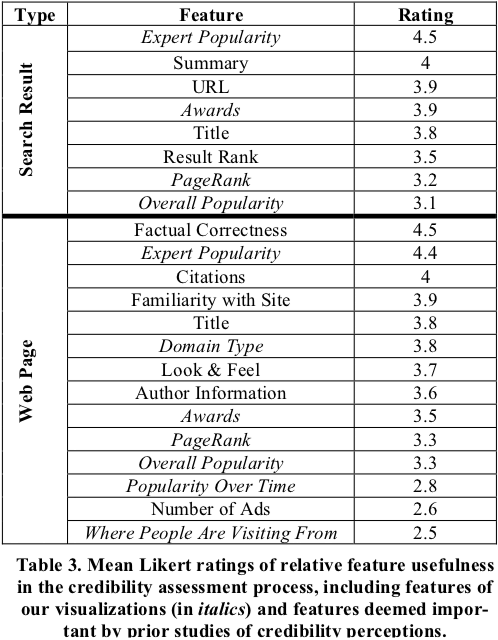
\includegraphics[scale=0.60]{results1.png}
\end{figure}

\subsection{Results}

Hypothesis and results:

\begin{itemize}
\item H1: Users’ credibility ratings will be more accurate when the visualizations are available to them. - yes
\item  H2: Users will feel more confident in the accuracy of their credibility ratings when the visualizations are available to them. - yes
\item H3: The impact (on both accuracy and confidence) of augmenting search results will be greater than the impact of augmenting Web pages. - accuracy but not confidence
\item H4: Teenagers’ ratings will receive more benefit from our intervention than adults’ will. - No
\end{itemize}

\section{Enhancing credibility judgment of web search results \cite{conf/chi/YamamotoT11}}

The aim of this paper is to bridge the gap between credibility theory in social psychology and search technology in Web information retrieval. The paper propose a system to help users judge the credibility of search results that Web search engines provide and find credible Web pages.

Information credibility is a \textit{subjective quality} that differs depending on the users and types of information . Therefore the system should judge the credibility of Web search results on the basis of users' credibility criteria.

Extension system for Web search engines (credibility-oriented Web searches):
\begin{itemize}
\item Analysis and visualization of scores of Web search results on the main credibility factors: accuracy, objectivity, authority, currency, and coverage. Each factor score is normalized by considering the distribution of the scores of all Web search results.

\item Prediction of users’ credibility judgment model through users’ credibility feedback for Web search results. Defined as user’s credibility judgment model as representation of how
important the user think each of main credibility aspects to judge the credibility of Web search results.

\item Re-ranking of Web search results based on a predicted users’ credibility model. To calculate credibility scores of Web search results, the system uses scores of each Web search result for each of five credibility aspects and the predicted users’ credibility judg-
ment model.

\end{itemize}

The goal of credibility-oriented Web searches is to obtain more credible Web pages from the large amount of Web  pages relevant to a given query.

\subsection{Features}

Main credibility factors:

\begin{itemize}
\item Accuracy \\
\textit{Referential importance} -  accurate Web pages are often linked to by
other Web pages as references; PageRank algorithm

\item Objectivity \\
\textit{Content typicality} - if a Web page is similar to many other Web
pages about a given query, the Web page is objective; LexRank algorithm 

\item Authority \\
\textit{Social reputation} - if a lot of people believe or highly regard certain Web pages, the Web pages are authoritative; social bookmarking websites

\item Currency \\
\textit{Freshness and update frequency} - Wayback Machine of Internet Archive (http://www.archive.org/web/web.php)

\item Coverage \\ 
\textit{Topic coverage} - number of technical terms in a page of the category; the algorithm is based on Wikipedia search 

\end{itemize}

\section{Ranking Comments on the Social Web  \cite{conf/cse/HsuKC09}}

One of the key features driving the growth and success of the Social Web is the large-scale user participation in content annotation via user-contributed tags, ratings, and comments.

The goal of the paper is to leverage these comments as a form of social collective intelligence for enhanced information organization, summarization, content retrieval, and visualization.

The paper propose a method to automatically rank the comments associated with a Social Web object (e.g., Web document, image, video) based on the expressed preferences of the community itself. By learning ranking functions for user contributed comments, it is possible to: (i) automatically score new comments as they arise in the community; (ii) promote highquality comments; (iii) filter out low-quality comments, so that user attention is not wasted; (iv) provide a sound basis for enhanced comment-based Social Web applications like summarization, content retrieval, visualization, and so on.

Challenges to comment ranking: short, lacking structure and links, link based quality metrics are impossible (e.g. Page Rank), quality assessment is relative to the object and its community, comments posed earlier may receive more attention, top-k comments for small k.

Regression-based learning approach for automatically ranking comments based on the expressed preferences of the community itself. The goal is to predict the relative order of comments, so that even as new ratings are made on the comments, the model will be able to capture the relative quality.

\subsection{Features} 

\begin{itemize}
\item \textit{Comment Visibility} - if more users in the community view a
comment, it is more likely to attract a larger community rating. Measured by two factores: (i) the \textit{article community rating} of the article that the comment is attached to; and (ii) the \textit{comment posting time}, since earlier comments may have the capacity to be viewed by more community members. In practice only the (ii) is possible.

\item \textit{User Reputation and Influence}

User’s activity and interest level within the community:
\begin{itemize}
\item Number of articles submitted
\item Community membership date
\item Category activity
\end{itemize}

User popularity in the community:
\begin{itemize}
\item Number of articles appearing on the Digg front page
\item Number of profile views
\item Number of friends
\end{itemize}

How well each user has participated in commenting in the past: 
\begin{itemize}
\item History of received comment ratings
\item History of received comment replies
\end{itemize}

\item \textit{Content-Based features}

Statistical properties of the text:
\begin{itemize}
\item Comment length
\item Comment complexity - measured by entropy:

\[
entropy(c_j) = \frac{1}{\lambda} \sum_{i=1}^{n} p_i[\log_{10} (\lambda) - \log_{10} (p_i)]
\]

\item Number of upper case words
\item Comment informativeness

\[
inform(c_j) = \sum_{t_i \in c_j} tf_{i,j} \times idf_i
\]

The $tf$ component values terms that occur frequently within a comment. The $idf$ component values terms that occur infrequently across comments.

\item Category cohesion - measured as sum of mutual information between the terms in the comment and the category $(cat)$ of the article.

\[
cohesion(c_j;cat) = \sum_{t \in c_j} MI(t,cat)
\]
\end{itemize}

NLP-style analysis of the comments:
\begin{itemize}
\item Readability - measured by its SMOG score, which estimates the years of
education needed to understand a piece of writing.
\item Subjectivity vs. objectivity
\item Verb+Noun count
\end{itemize}

Compare the comment text to the article the comment is attached to:
\begin{itemize}
\item Comment-article overlap
\item Comment-article polarity
\end{itemize}

\end{itemize}

\begin{figure}[!htb]
  \centering
  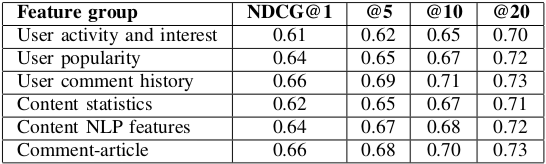
\includegraphics[scale=0.60]{results2.png}
\end{figure}

\begin{figure}[!htb]
  \centering
  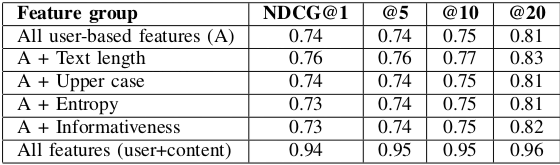
\includegraphics[scale=0.60]{results3.png}
\end{figure}

\bibliography{references}{}
\bibliographystyle{plain}

\end{document}